\documentclass[10pt]{article}
\usepackage[paper=letterpaper,margin=2cm]{geometry}
\usepackage{amsmath}
\usepackage{amssymb}
\usepackage{amsfonts}
\usepackage{newtxtext, newtxmath}
\usepackage{enumitem}
\usepackage{titling}
\usepackage{graphicx}    %  in the preamble
\usepackage{fancyhdr}
\usepackage{subcaption}
\usepackage[colorlinks=true]{hyperref}

\setlength{\droptitle}{-10em}

\fancyhf{}
\fancyhead[L]{MATH 232: Linear Algebra}
\fancyhead[R]{Steven Wong, 301337727}
\renewcommand\headrulewidth{0pt}
\pagestyle{fancy}

\begin{document}

\noindent\makebox[\textwidth][c]{\Large\bfseries Assignment 3: Population Dynamics}
\normalsize
\begin{enumerate}[leftmargin=\labelsep]
    \item 
    To find the \href{https://www150.statcan.gc.ca/t1/tbl1/en/tv.action?pid=1710000501}{age distribution}, \href{https://www150.statcan.gc.ca/t1/tbl1/en/tv.action?pid=1310041801}{birth rate}, 
    and \href{https://www150.statcan.gc.ca/t1/tbl1/en/tv.action?pid=1310071001}{morality rates} for the Canadian population, I gathered data from Statistics Canada's website where time
    $t_0$ was set to the year $2020$, as this is the most recent year for which data is available for all three of these variables. In order to
    create 100 bin vectors, I assumed that the distribution of the data was uniform over each of the defined age groups. For example, the population 
    of age group $0-4$ was $1,918,870$ people, and therefore, each bin should have a value of $\frac{1,918,870}{5} = 383,774$ people. Calculations for the birth and mortality rates
     follow similarly.
        
    \item How do I "specify" my 100*100 transition matrix in a one page report? Similarly to the discrete dynamical model described by Boyd and 
    Vandenberghe, the birth rate was given by a 100-vector b where $b_i$ is the average births per person with age $i-1$. The mortality
    rate is given by a 100-vector d, where $d_i$ is the portion of people aged $i-1$ who die in the current year. Then the transition matrix
    is given by A where the first row is $b_0$ to $b_{99}$ and subsequent rows are given by $1-d_i$ along the diagonal.
    
    \item Using the initial population vector given by my 2020 age distribution, and the transition matrix given by my birth and mortality rates, 
    I projected the population of Canada for the years 2028, 2033, and 2038. These results were found by repeatingly multiplying the population vector
    by the transition matrix in a for loop. The results are shown in the figure below.

    \begin{figure}[h]
        \centering
        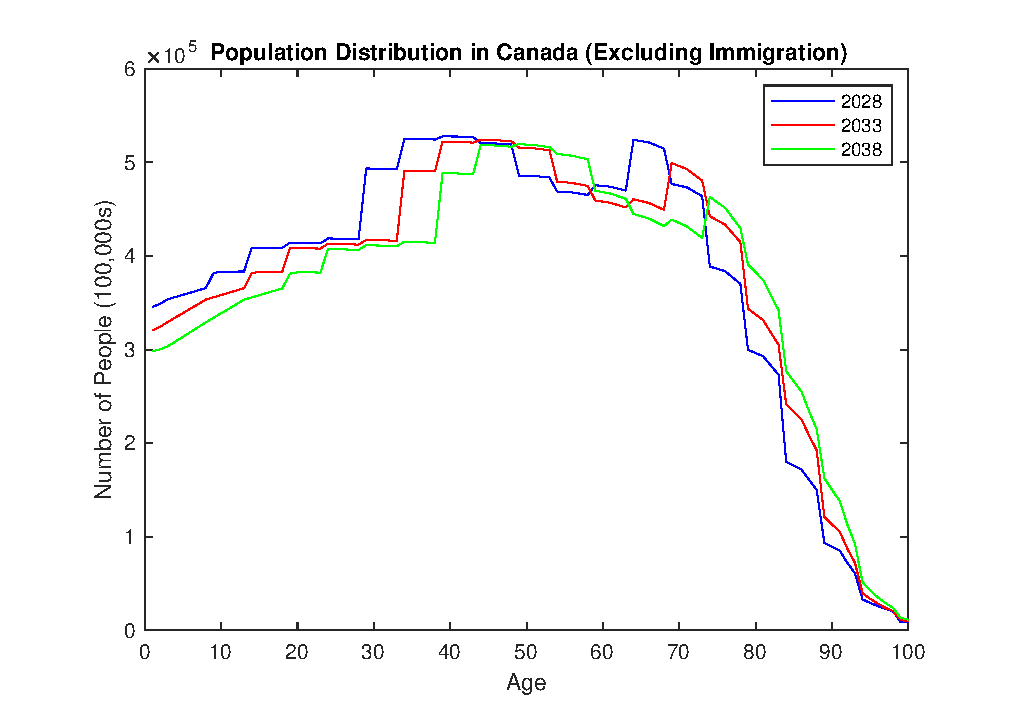
\includegraphics{WithoutImmigration.eps}
        \caption{Caption}
        \label{fig:my_label}
    \end{figure}
    
    \item \textbf{Make a modification of the model to incorporate immigration using a simple assumption of the average immigration rate. Plot the predicted age distribution for the years 2028, 2033, and 2038.}
    I gathered immigration data from Statistics Canada "Estimates of the components of international migration, by age and sex, annual"
    for the 2021/2022 year and created a 100 bin vector similar to the age distribution. I treated this immigration factor as an exogenous
    variable, adding it to the results of each iteration in the for loops described in question 3. In these projections, I assumed that 
    the immigration rates through to 2038 would remain constant at the 2021/2022 rate. The results are shown in the figure below:
    
    \begin{figure}[h]
        \centering
        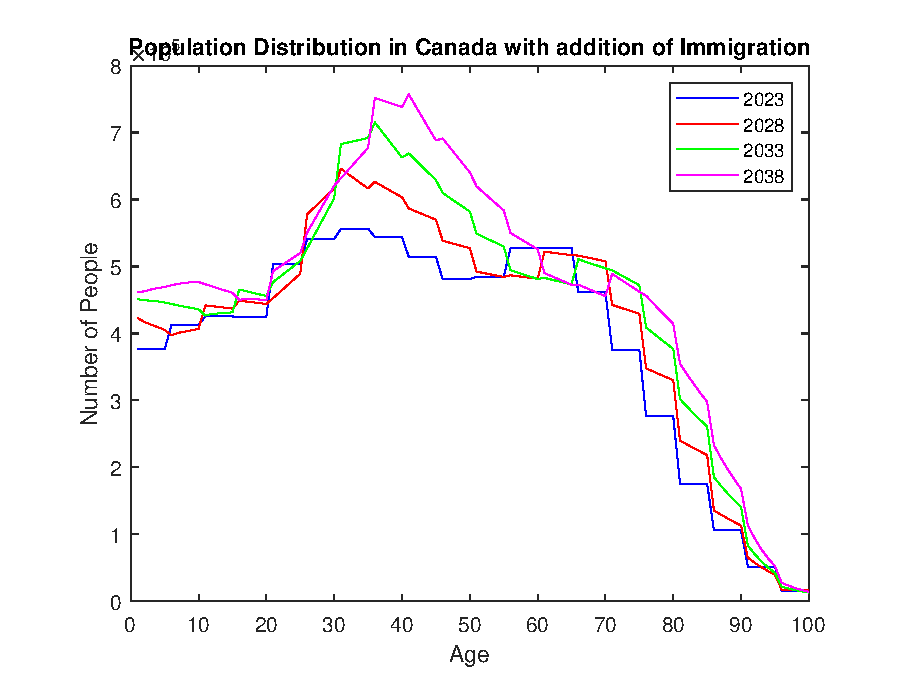
\includegraphics{WithImmigration.eps}
        \caption{Caption}
        \label{fig:my_label}
    \end{figure}
    
    \item \textbf{What other factors do you think would make this model more accurate?} 
    If we were to make the model more realistic, we would have to take into account the fact that the population is not evenly distributed across the age groups.
    Furthermore, we could also take into account the fact that fertility, mortality, and immigration rates are not constant over time and vary based on external factors.
\end{enumerate}
\end{document}